\documentclass[11pt,a4paper,english]{uvamath}
\usepackage[english]{babel}

\usepackage{amsmath, amsfonts, amssymb, a4wide, fancyhdr, lineno, graphicx, epsfig, soul, color, hyperref}
\usepackage[square, numbers]{natbib}

% Running line numbers:
\linenumbers
% Number only every 5:th line:
\modulolinenumbers[5]

%Nodig om een bibliography midden in het artikel te zetten, ipv aan het einde zoals eigenlijk gebruikelijk is
\renewcommand{\bibsection}{}

% TODO command
\newcommand{\todo}[1]{
    \hl{#1}
}

% The things that should be filled in by each group, depending on their situation, are written in a todo command, \todo{like this text}. All text in normal the normal font, is applicable for any group. However, everyone is free to adapt any text, and it is even suggested to look at all text critically and make changes if needed.

% Project specific commands
\author{Tom van Duist \& Kevin van den Bekerom}

\newcommand{\projectname}{\todo{Project Name}\ }


\newcommand{\aanpassen}[1]{ {\sethlcolor{green} \hl{#1}} }

\title{Requirements Document}
%Variables
\newcommand{\TitelAbbr}{RD}
\newcommand{\Version}{0.1}



\what{Lab assignment Requirements Engineering}
\supervisors{}

\coverimage{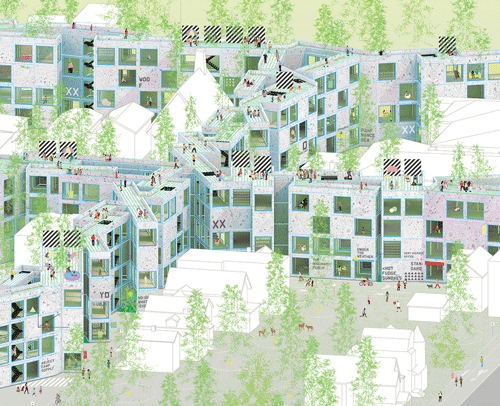
\includegraphics[scale=0.5]{Images/titleImage}\\
"\emph{The architecture giveth and the implementation taketh away.}"\\ - Len Bass, Paul Clements, Rick Kazman}


\begin{document}

\maketitle


\tableofcontents

\chapter*{Document Status Sheet}
\section*{Document status overview}
\subsection*{General}
\begin{tabular}[!]{ll}
    Document title:     & Architectural Design Document\\
    Authors:           	& Kevin van den Bekerom \\ 
						& Tom van Duist \\
    Document status:    & Draft release\\
\end{tabular}

\subsection*{Document history}
\begin{tabular}[!]{|l|l|l|l|}
    \hline
    \emph{Version}    &   \emph{Date} &  \emph{Reason of change}\\
    \hline
    0.0 & 02-09-2015 &  Setup of the document layout\\    
    \hline
    0.1 & 29-10-2015 & Release version week 1 \\
    \hline
\end{tabular}

\clearpage

%\section*{Document Change Records since previous issue}
%\subsection*{General}
%\begin{tabular}[!]{ll}
%   Datum:          &   2015-06-09 \\
%    Document title: &   Architectural Design Document (ADD)\\
%    Identification:  &   \TitelAbbr\_\Version.pdf\\
%\end{tabular}

%\subsection*{Changes}
%\begin{tabular}[!]{|l|l|p{8 cm}|}
%    \hline
%    \emph{Chapter} &   \emph{Paragraph}    &   \emph{Reason to change}\\
%    \hline
%    \ref{c:main_fun} &  whole chapter      & Make prioritizing clear using Moscov model. Clarified functionalities. \\
%    \hline
%    dfdf& tt & ff. \\
%    \hline
%\end{tabular} 

\chapter{Introduction}
Blabla.

\chapter{Project Plan}
The project plan for the first four weeks is explained in this chapter. The goal is to discover the services to be provided by the successor of Blackboard. We base our project plan on the requirements lifecycle in \cite{RE_book} (chapter 1.1.6). This book identifies four phases of requirements engineering; 
\begin{enumerate}
	\item Domain understanding and elicitation.
	\item Evaluation and negotiation.
	\item Specification and documentation.
	\item Quality assurance.
\end{enumerate}

During the first week we will get familiar with the problem world, as described in \cite{RE_book}. We will investigate the system-as-is ourselves, and ask users (students) about their experiences. We will work trough the questions listed in the relevant section in the book. We will also compose a list of stakeholders, which we interview in the coming weeks.

Week 2 will resolve around the second phase: evaluation and negotiation. During this week we will interview remaining stakeholders, to verify and add upon the information we gathered in the first week. Interviewing all relevant stakeholders is crucial during this week, as it is a required input to this the evaluation and negotiation phase, and subsequent phases. Due to limited time we can interview maximally 3 stakeholders per group. If a stakeholder is not readily available we will not use his/her input in the requirements engineering process. 

During week 3 we will draft an initial set of requirements. After week 3 the first draft version of the Requirements Document is finished. We will focus on the smallest set of requirements that together realize (most of) the business goals, due to limited time. 

In week 4 we will plan meetings with relevant stakeholders to asses the set of requirements we drafted for the new system. Assessment focuses on whether we forgot crucial requirements and if the requirements are consistent.  

\chapter{Domain Analysis}

\section{Glossary of terms}
\todo{List all relevant terms in the problem world}

\section{Organization}
The organization in which Blackboard is used is the University of Amsterdam (UvA). 

The organization within which the system-as-is takes place: its structure, strategic objectives,
business policies, roles played by organizational units and actors, and dependencies
among them.

\section{Scope}
The scope of the system-as-is: its underlying objectives, the components forming it, the
concepts on which it relies, the tasks involved in it, the information flowing through it,
and the constraints and regulations to which the system is subject.

\section{Stakeholders}
\begin{itemize}
	\item Users: Both students and teachers
	\item Management:
	\item Blackboard (company):
\end{itemize}

The set of stakeholders to be involved in the RE process.

\section{Strengths and Weaknesses}
Students:
\begin{itemize}
	\item[+] Easy way to access course specific information.
	\item[+] Latest schedule of course.
	\item[-] Hard to use in the beginning.
	\item[-] Only marginal functionality used, e.g. "We \textit{have} to use it."
\end{itemize}



The strengths and weaknesses of the system-as-is, as perceived by the identified stakeholders.

\section{Domain facts}


\chapter{References}

\begin{thebibliography}{9}
	
	\bibitem{bosch}
	Jan Bosch,
	\emph{Software Architecture: The Next Step},
	University of Groningen, Department of Computing Science
	
	\bibitem{RE_book}
	Axel van Lamsweerde,
	\emph{Requirements Engineering: From System Goals to UML Models to Software Specifications}
	
	
\end{thebibliography}


\appendix


\end{document}
